\documentclass[fontset=windows, chinese, 10pt, xcolor=dvipsnames]{beamer}

\usepackage{amsmath,amssymb,mathtools}
\usepackage{xeCJK}
\usepackage{zhnumber}
\usepackage{tikz}
\usetikzlibrary{quotes,angles,arrows.meta,calc}

\usetheme{metropolis}
\usepackage{beamercolorthemeHistNanjing}

\newcommand{\red}[1]{\textcolor{red}{#1}}
\newcommand{\blue}[1]{\textcolor{blue}{#1}}
\newcommand{\green}[1]{\textcolor{green}{#1}}
\newcommand{\gray}[1]{\textcolor{gray}{#1}}
\newcommand{\orange}[1]{\textcolor{orange}{#1}}

\newcommand{\vecfig}[1]{%
  \IfFileExists{tikz/#1.tex}%
    {\input{tikz/#1.tex}}%
    {\input{../../lecture_new/chapters/vec/tikz/#1.tex}}}

\newcommand{\sssub}[1]{ {\mathrm{#1} }}  % script size subscript\\\
\newcommand{\funcd}[2]{ \frac{d{#1}}{d{#2}}} %function full derivative
\newcommand{\funcpd}[2]{ \frac{\partial{#1}}{\partial{#2}}} %function partial derivative
\newcommand{\fnald}[2] { \frac{\delta {#1}}{\delta {#2}}} % functional derivative

\renewcommand{\Re}{\operatorname{Re}}
\renewcommand{\Im}{\operatorname{Im}}
\def\ext{\sssub{ext}}
\def\x{\sssub{x}}
\def\xc{\sssub{xc}}
\def\H{\sssub{H}}
\def\Hx{\sssub{Hx}}
\def\Hxc{\sssub{Hxc}}
\def\c{\sssub{c}}
\def\s{\sssub{s}}

% \def\ext{\sssub{ext}}
% \def\ext{\sssub{ext}}
% \def\ext{\sssub{ext}}
% \def\ext{\sssub{ext}}
% \defsssub{ext}


% definitions of bold faced symbols
\def\brpppp{{\mathbf{r}^{\prime\prime\prime\prime}}}
\def\brppp{{\mathbf{r}^{\prime\prime\prime}}}
\def\brpp{{\mathbf{r}^{\prime\prime}}}
\def\brp{{\mathbf{r}^{\prime}}}
\def\bzp{{\mathbf{z}^{\prime}}}
\def\bxp{{\mathbf{x}^{\prime}}}
\def\tp{{{t}^{\prime}}}
\def\tpp{{{t}^{\prime\prime}}}
\def\tppp{{{t}^{\prime\prime\prime}}}

\def\tbr{{\tilde{\mathbf{r}}}}
\def\bk{{\mathbf{k}}}
\def\br{{\mathbf{r}}}
\def\bp{{\mathbf{p}}}
\def\bq{{\mathbf{q}}}
\def\bv{{\mathbf{v}}}
\def\bz{{\mathbf{z}}}
\def\mbf{{\mathbf{f}}}

\def\bx{{\mathbf{x}}}
\def\bR{{\mathbf{R}}}
\def\bM{{\mathbf{M}}}
\def\bP{{\mathbf{P}}}
\def\bT{{\mathbf{T}}}
\def\bK{{\mathbf{K}}}
\def\bA{{\mathbf{A}}}
\def\bB{{\mathbf{B}}}
\def\bD{{\mathbf{D}}}
\def\bE{{\mathbf{E}}}
\def\bF{{\mathbf{F}}}
\def\bG{{\mathbf{G}}}
\def\bH{{\mathbf{H}}}
\def\bI{{\mathbf{I}}}
\def\bJ{{\mathbf{J}}}
\def\bP{{\mathbf{P}}}
\def\bS{{\mathbf{S}}}
\def\bV{{\mathbf{V}}}
\def\bX{{\mathbf{X}}}
\def\bY{{\mathbf{Y}}}
\def\dd{{\mathop{}\!\mathrm{d}}}
\def\dr{{\!\!\dd\br\,}}
\def\dx{{\!\!\dd\bx\,}}
\def\dy{{\!\!\dd\by\,}}
\def\dk{{\!\!\dd\bk\,}}
\def\dG{{\!\!\dd\bG\,}}


\def\half{{\frac{1}{2}}}
\def\tr{{\mathrm{tr}}}


\def\Arg{{\mathrm{Arg}\;}}
\def\arg{{\mathrm{arg}\;}}
\def\Res{{\mathrm{Res}\;}}


\title{矢量分析}
\subtitle{第三讲：指标记号与张量}


\date{\zhdigits{\the\year},\zhganzhinian{\the\year}年秋}
\author{罗凯}
\institute{南京理工大学物理学院}

\usebackgroundtemplate{%
\begin{tikzpicture}[remember picture,overlay]
  \node[opacity=0.05, at=(current page.center)] {
    
\includegraphics[width=0.6\paperwidth]{njust-logo.jpeg}
  };
\end{tikzpicture}}
\begin{document}

\begin{frame}
  \titlepage
\end{frame}

\AtBeginSubsection{
  \begin{frame}{提纲}
    \tableofcontents[currentsection,currentsubsection]
  \end{frame}
}

\begin{frame}
  \titlepage
\end{frame}

\AtBeginSubsection{
  \begin{frame}{提纲}
    \tableofcontents[currentsection,currentsubsection]
  \end{frame}
}

\section{指标记号}

\subsection{求和约定}

\begin{frame}{$\mathbb{R}^n$ 中的矢量}
  同一套想法从三维自然延伸到 $\mathbb{R}^n$。
  $n$ 维矢量是分量的有序数组，
  \begin{equation*}
    \mathbf{v}
    =(v_1,\ldots,v_n)
    =\sum_{i=1}^{n}v_i\mathbf{e}_i,
  \end{equation*}
  其中 $\{\mathbf{e}_1,\ldots,\mathbf{e}_n\}$ 是正交归一的直角基。
  两点的坐标是 $(x_1,\ldots,x_n)$。
  两个矢量相等，当且仅当每一个对应分量都相等。
  矩阵 $M$ 第 $i$ 行第 $j$ 列的元素记为 $M_{ij}$。
\end{frame}

\begin{frame}{爱因斯坦求和约定}
  一个指标在同一项里恰好出现两次，就对该指标的全部取值求和，求和号省去：
  \begin{align*}
    \mathbf{u}\cdot\mathbf{v}
    &=\sum_{i=1}^{n}u_i v_i
     =u_i v_i,\\[0.4em]
    [AB]_{ij}
    &=\sum_{k=1}^{n}A_{ik}B_{kj}
     =A_{ik}B_{kj}.
  \end{align*}
  \begin{itemize}
    \item \textbf{哑指标}被求和，可以改名。
    \item \textbf{自由指标}在每一项里出现一次，必须原样保留。
  \end{itemize}
\end{frame}

\begin{frame}{改名与禁例}
  哑指标改名不改变这一项，自由指标保持不变：
  \begin{equation*}
    A_{ik}B_{kl}C_{lj}
    =A_{im}B_{ml}C_{lj}.
  \end{equation*}
  两边的自由指标都是 $i$ 与 $j$。
  \vspace{0.5em}
  \begin{alertblock}{每个指标出现一次或两次}
    $A_{ik}B_{kk}C_{kj}$ 不合法，因为 $k$ 出现了三次。
    一项之中，任何一个指标不得出现两次以上。
  \end{alertblock}
\end{frame}

\begin{frame}{克罗内克符号}
  克罗内克 $\delta$ 是单位矩阵的分量：
  \begin{equation*}
    \delta_{ij}
    =
    \begin{cases}
      1, & i=j,\\
      0, & i\neq j.
    \end{cases}
  \end{equation*}
  三条常用缩并是
  \begin{equation*}
    \delta_{ij}a_j=a_i,
    \qquad
    \delta_{ij}\delta_{jk}=\delta_{ik},
    \qquad
    \delta_{ii}=n.
  \end{equation*}
  下面把三条都证出来。
\end{frame}

\begin{frame}{证明三条缩并}
  对固定的 $i$，求和 $\delta_{ij}a_j$ 里只有 $j=i$ 的那一项不为零，所以等于 $a_i$。
  \vspace{0.4em}
  同样，$\delta_{ij}\delta_{jk}$ 里只有 $j=i$ 存活，得到 $\delta_{ik}$。
  \vspace{0.4em}
  最后 $\delta_{ii}=\sum_{i=1}^{n}\delta_{ii}$。
  对角线上有 $n$ 个 $1$，所以 $\delta_{ii}=n$。
\end{frame}

\begin{frame}{列维-奇维塔符号}
  三维完全反对称符号定义为
  \begin{equation*}
    \varepsilon_{ijk}
    =
    \begin{cases}
      +1, & (i,j,k)\ \text{是}\ (1,2,3)\ \text{的偶置换},\\
      -1, & (i,j,k)\ \text{是}\ (1,2,3)\ \text{的奇置换},\\
      0, & \text{其余情形，即有重复指标}.
    \end{cases}
  \end{equation*}
  因此
  $\varepsilon_{123}=\varepsilon_{231}=\varepsilon_{312}=1$，
  $\varepsilon_{132}=\varepsilon_{213}=\varepsilon_{321}=-1$。
\end{frame}

\begin{frame}{交换两个指标变号}
  设 $(i,j,k)$ 是 $(1,2,3)$ 的一个置换，符号为 $s=\varepsilon_{ijk}$。
  对换其中任意两个指标，置换的奇偶性改变，符号从 $s$ 变成 $-s$。
  若原来已有重复指标，则 $\varepsilon_{ijk}=0$，对换之后仍然有重复指标，仍是 $0$。
  所以在一切情形下
  \begin{equation*}
    \varepsilon_{ijk}=-\varepsilon_{jik}
    =-\varepsilon_{ikj}
    =-\varepsilon_{kji}.
  \end{equation*}
\end{frame}

\begin{frame}{由此得到 $\mathbf{u}\times\mathbf{u}=\mathbf{0}$}
  叉积的指标形式是
  $(\mathbf{u}\times\mathbf{u})_i=\varepsilon_{ijk}u_j u_k$。
  把哑指标 $j,k$ 对换：
  \begin{equation*}
    \varepsilon_{ijk}u_j u_k
    =\varepsilon_{ikj}u_k u_j
    =-\varepsilon_{ijk}u_j u_k,
  \end{equation*}
  这里用了 $u_j u_k=u_k u_j$ 以及 $\varepsilon_{ikj}=-\varepsilon_{ijk}$。
  一个数等于自己的相反数，所以
  \begin{equation*}
    \varepsilon_{ijk}u_j u_k=0,
    \qquad
    \mathbf{u}\times\mathbf{u}=\mathbf{0}.
  \end{equation*}
\end{frame}

\subsection{乘积与导数}

\begin{frame}{线性代数的指标形式}
  方程组 $A\mathbf{x}=\mathbf{b}$ 写成 $A_{ij}x_j=b_i$。
  本征对用 $\alpha$ 编号，$\alpha$ 不参与求和：
  \begin{equation*}
    A_{ij}v_j^{(\alpha)}
    =\lambda^{(\alpha)}v_i^{(\alpha)},
    \qquad \alpha=1,\ldots,n.
  \end{equation*}
  正交矩阵满足 $R_{ki}R_{kj}=\delta_{ij}$。
  迹是 $\operatorname{tr}A=A_{ii}$。
  标量乘法可交换，所以迹有循环性：
  \begin{equation*}
    \operatorname{tr}(AB)
    =A_{ij}B_{ji}
    =B_{ji}A_{ij}
    =\operatorname{tr}(BA).
  \end{equation*}
\end{frame}

\begin{frame}{例：平面旋转}
  \begin{equation*}
    R=
    \begin{pmatrix}
      \cos\theta & -\sin\theta \\
      \sin\theta & \cos\theta
    \end{pmatrix}.
  \end{equation*}
  $R^{\mathsf T}R$ 的 $11$ 分量：
  \begin{align*}
    R_{k1}R_{k1}
    &= R_{11}R_{11}+R_{21}R_{21} \\
    &= \cos^2\theta+\sin^2\theta
     = 1.
  \end{align*}
  $12$ 分量：
  \begin{align*}
    R_{k1}R_{k2}
    &= \cos\theta(-\sin\theta)+\sin\theta\cos\theta
     = 0.
  \end{align*}
  $21$、$22$ 同样得到 $\delta_{ij}$，所以 $R_{ki}R_{kj}=\delta_{ij}$。
\end{frame}

\begin{frame}{正交变换保持内积}
  设 $(R\mathbf{u})_i=R_{ij}u_j$。由 $R_{ki}R_{kj}=\delta_{ij}$，
  \begin{align*}
    (R\mathbf{u})\cdot(R\mathbf{v})
    &= (R_{ik}u_k)(R_{il}v_l)
     = R_{ik}R_{il}\, u_k v_l \\
    &= \delta_{kl}u_k v_l
     = u_k v_k
     = \mathbf{u}\cdot\mathbf{v}.
  \end{align*}
  取 $\mathbf{v}=\mathbf{u}$，得到 $|R\mathbf{u}|=|\mathbf{u}|$。
  长度与内积都不变，夹角
  $\cos\theta=(\mathbf{u}\cdot\mathbf{v})/(|\mathbf{u}|\,|\mathbf{v}|)$
  也不变。
\end{frame}

\begin{frame}{点积与叉积}
  \begin{equation*}
    \mathbf{u}\cdot\mathbf{v}
    =u_i v_i
    =\delta_{ij}u_i v_j,
  \end{equation*}
  \begin{equation*}
    (\mathbf{u}\times\mathbf{v})_i
    =\varepsilon_{ijk}u_j v_k.
  \end{equation*}
  后一式就是行列式展开：
  $i=1$ 时 $\varepsilon_{1jk}u_j v_k=u_2 v_3-u_3 v_2$，
  与 $\mathbf{e}_x$ 分量一致。
\end{frame}

\begin{frame}{标量三重积}
  从叉积出发，
  \begin{align*}
    \mathbf{u}\cdot(\mathbf{v}\times\mathbf{w})
    &= u_i(\mathbf{v}\times\mathbf{w})_i
     = u_i\varepsilon_{ijk}v_j w_k
     = \varepsilon_{ijk}u_i v_j w_k.
  \end{align*}
  把哑指标循环改名 $(i,j,k)\to(j,k,i)$。
  这是偶置换，$\varepsilon_{jki}=\varepsilon_{ijk}$，于是
  \begin{equation*}
    \varepsilon_{ijk}u_i v_j w_k
    =\varepsilon_{jki}u_j v_k w_i
    =\mathbf{v}\cdot(\mathbf{w}\times\mathbf{u}).
  \end{equation*}
  再循环一次得到 $\mathbf{w}\cdot(\mathbf{u}\times\mathbf{v})$。
  对换 $\mathbf{v}$ 与 $\mathbf{w}$ 使 $\varepsilon_{ijk}$ 在后两个指标上变号，所以三重积变号。
\end{frame}

\begin{frame}{$\varepsilon$--$\delta$ 恒等式}
  \begin{equation*}
    \varepsilon_{ijk}\varepsilon_{klm}
    =\delta_{il}\delta_{jm}-\delta_{im}\delta_{jl}.
  \end{equation*}
  证明分三步。
  \begin{enumerate}
    \item $i=j$ 时左边有重复指标，为零；右边两项相同，也为零。$l=m$ 时同样。
    \item 两边都对 $(i,j)$ 和 $(l,m)$ 反对称，所以只要核对 $(i,j)=(1,2)$。
    \item $(i,j)=(1,2)$ 时只有 $k=3$ 有贡献：
      $\varepsilon_{123}\varepsilon_{3lm}=\varepsilon_{3lm}$。
      它在 $(l,m)=(1,2)$ 时为 $1$，在 $(2,1)$ 时为 $-1$，其余为零。
      右边 $\delta_{1l}\delta_{2m}-\delta_{1m}\delta_{2l}$ 给出同一组值。
  \end{enumerate}
  其他指标对由反对称性带上同一个符号，恒等式成立。
\end{frame}

\begin{frame}{矢量三重积}
  \begin{align*}
    \bigl[\mathbf{u}\times(\mathbf{v}\times\mathbf{w})\bigr]_i
    &= \varepsilon_{ijk}u_j(\varepsilon_{klm}v_l w_m) \\
    &= \varepsilon_{ijk}\varepsilon_{klm}\, u_j v_l w_m \\
    &= (\delta_{il}\delta_{jm}-\delta_{im}\delta_{jl})
       u_j v_l w_m \\
    &= u_j v_i w_j - u_j v_j w_i \\
    &= (\mathbf{u}\cdot\mathbf{w})v_i
     - (\mathbf{u}\cdot\mathbf{v})w_i.
  \end{align*}
  写回矢量，
  \begin{equation*}
    \mathbf{u}\times(\mathbf{v}\times\mathbf{w})
    =(\mathbf{u}\cdot\mathbf{w})\mathbf{v}
    -(\mathbf{u}\cdot\mathbf{v})\mathbf{w}.
  \end{equation*}
\end{frame}

\begin{frame}{进一步的缩并}
  计算 $\varepsilon_{ijk}\varepsilon_{ljk}$，其中 $j,k$ 求和。
  \vspace{0.3em}
  若 $i\neq l$，例如 $i=1$、$l=2$，则对每一个 $(j,k)$，
  $\varepsilon_{1jk}$ 与 $\varepsilon_{2jk}$ 至少有一个因指标重复而为零，所以缩并是 $0$。
  \vspace{0.3em}
  若 $i=l=1$，非零项只有两对：
  \begin{align*}
    (j,k)=(2,3):&\quad \varepsilon_{123}\varepsilon_{123}=1,\\
    (j,k)=(3,2):&\quad \varepsilon_{132}\varepsilon_{132}=1.
  \end{align*}
  和为 $2$。$i=l=2$ 与 $i=l=3$ 同样得 $2$。
  因此
  \begin{equation*}
    \varepsilon_{ijk}\varepsilon_{ljk}=2\delta_{il}.
  \end{equation*}
\end{frame}

\begin{frame}{完全缩并}
  在上式中令 $l=i$ 并对 $i$ 求和：
  \begin{equation*}
    \varepsilon_{ijk}\varepsilon_{ijk}
    =2\delta_{ii}
    =2n.
  \end{equation*}
  三维中 $n=3$，所以
  \begin{equation*}
    \varepsilon_{ijk}\varepsilon_{ijk}=6=3!.
  \end{equation*}
  $3!$ 是 $\{1,2,3\}$ 的全部置换个数，每一个置换对完全缩并贡献 $1$。
\end{frame}

\begin{frame}{$\varepsilon_{ijk}\delta_{jk}=0$}
  $\delta_{jk}$ 只留下 $j=k$ 的项，而 $\varepsilon_{ijj}=0$。
  同一结论来自对称性：$\delta_{jk}$ 对 $(j,k)$ 对称，$\varepsilon_{ijk}$ 对 $(j,k)$ 反对称，二者缩并为零。
\end{frame}

\begin{frame}{导数与真空麦克斯韦方程}
  把 $\partial/\partial x_i$ 写成 $\partial_i$。
  \begin{align*}
    \nabla\cdot\mathbf{E}=0
    &\longrightarrow \partial_i E_i=0,\\
    \nabla\cdot\mathbf{B}=0
    &\longrightarrow \partial_i B_i=0,\\
    \nabla\times\mathbf{E}+\partial_t\mathbf{B}=\mathbf{0}
    &\longrightarrow
      \varepsilon_{ijk}\partial_j E_k+\partial_t B_i=0,\\
    \nabla\times\mathbf{B}
    -\mu_0\varepsilon_0\partial_t\mathbf{E}=\mathbf{0}
    &\longrightarrow
      \varepsilon_{ijk}\partial_j B_k
      -\mu_0\varepsilon_0\partial_t E_i=0.
  \end{align*}
  散度是 $\partial_i$ 与场的重复指标，旋度是 $\varepsilon_{ijk}\partial_j$ 作用在场上。
\end{frame}

\begin{frame}{梯度的旋度}
  \small
  \begin{align*}
    (\nabla\times\nabla\varphi)_i
    &= \varepsilon_{ijk}\partial_j\partial_k\varphi \\
    &= \varepsilon_{ijk}\partial_k\partial_j\varphi
      && \text{（混合偏导可交换）}\\
    &= -\varepsilon_{ikj}\partial_k\partial_j\varphi
      && \text{（$\varepsilon_{ijk}$ 反对称）}\\
    &= -(\nabla\times\nabla\varphi)_i.
  \end{align*}
  \normalsize
  因此 $\nabla\times\nabla\varphi=\mathbf{0}$。
  对乘积 $f\mathbf{A}$，同样的反对称性配合求导的乘积法则，用在后面的矢量恒等式里。
\end{frame}

\begin{frame}{旋度的旋度}
  \begin{align*}
    \bigl[\nabla\times(\nabla\times\mathbf{E})\bigr]_i
    &= \varepsilon_{ijk}\partial_j(\varepsilon_{klm}\partial_l E_m) \\
    &= (\delta_{il}\delta_{jm}-\delta_{im}\delta_{jl})
       \partial_j\partial_l E_m \\
    &= \partial_i(\partial_j E_j)
     - \partial_j\partial_j E_i.
  \end{align*}
  写回矢量，
  \begin{equation*}
    \nabla\times(\nabla\times\mathbf{E})
    =\nabla(\nabla\cdot\mathbf{E})-\nabla^2\mathbf{E}.
  \end{equation*}
\end{frame}

\begin{frame}{$\nabla\cdot(\nabla\times\mathbf{u})=0$}
  \begin{align*}
    \partial_i(\nabla\times\mathbf{u})_i
    &= \partial_i(\varepsilon_{ijk}\partial_j u_k)
     = \varepsilon_{ijk}\partial_i\partial_j u_k.
  \end{align*}
  $\partial_i\partial_j$ 对 $(i,j)$ 对称，$\varepsilon_{ijk}$ 对 $(i,j)$ 反对称，缩并为零。
  把哑指标对换也能写成一项等于自己的相反数。
\end{frame}

\begin{frame}{$\mathbf{u}\times(\nabla\times\mathbf{u})$}
  \small
  \begin{align*}
    \bigl[\mathbf{u}\times(\nabla\times\mathbf{u})\bigr]_i
    &= \varepsilon_{ijk}u_j(\varepsilon_{klm}\partial_l u_m) \\
    &= (\delta_{il}\delta_{jm}-\delta_{im}\delta_{jl})
       u_j\partial_l u_m \\
    &= u_j\partial_i u_j - u_j\partial_j u_i \\
    &= \partial_i\Bigl(\frac12 u_j u_j\Bigr)
     - \bigl[(u\cdot\nabla)\mathbf{u}\bigr]_i.
  \end{align*}
  \normalsize
  中间一步用了
  $\partial_i(u_j u_j)=2u_j\partial_i u_j$。
  所以
  \begin{equation*}
    \mathbf{u}\times(\nabla\times\mathbf{u})
    =\nabla\Bigl(\frac12|\mathbf{u}|^2\Bigr)
    -(\mathbf{u}\cdot\nabla)\mathbf{u}.
  \end{equation*}
\end{frame}

\begin{frame}{$\nabla\cdot(\mathbf{u}\times\mathbf{v})$}
  乘积法则：
  \begin{equation*}
    \partial_i(\varepsilon_{ijk}u_j v_k)
    =\varepsilon_{ijk}(\partial_i u_j)v_k
    +\varepsilon_{ijk}u_j\partial_i v_k.
  \end{equation*}
  第一项把指标改名为 $\varepsilon_{lmk}v_k\partial_l u_m$。
  循环 $(l,m,k)\to(k,l,m)$ 是偶置换，所以
  $\varepsilon_{lmk}=\varepsilon_{klm}$，第一项等于
  $v_k(\nabla\times\mathbf{u})_k$。
  第二项 $\varepsilon_{ijk}=-\varepsilon_{jik}$，等于
  $-\,u_j(\nabla\times\mathbf{v})_j$。
  因此
  \begin{equation*}
    \nabla\cdot(\mathbf{u}\times\mathbf{v})
    =\mathbf{v}\cdot(\nabla\times\mathbf{u})
    -\mathbf{u}\cdot(\nabla\times\mathbf{v}).
  \end{equation*}
\end{frame}

\begin{frame}{$\nabla\times(\mathbf{u}\times\mathbf{v})$}
  \small
  \begin{align*}
    \bigl[\nabla\times(\mathbf{u}\times\mathbf{v})\bigr]_i
    &= \varepsilon_{ijk}\partial_j(\varepsilon_{klm}u_l v_m) \\
    &= (\delta_{il}\delta_{jm}-\delta_{im}\delta_{jl})
       \partial_j(u_l v_m) \\
    &= \partial_j(u_i v_j)-\partial_j(u_j v_i) \\
    &= (\partial_j u_i)v_j+u_i\partial_j v_j
     - (\partial_j u_j)v_i-u_j\partial_j v_i.
  \end{align*}
  \normalsize
  四项依次是
  $[(\mathbf{v}\cdot\nabla)\mathbf{u}]_i$、
  $u_i(\nabla\cdot\mathbf{v})$、
  $-v_i(\nabla\cdot\mathbf{u})$、
  $-[(\mathbf{u}\cdot\nabla)\mathbf{v}]_i$。
\end{frame}

\begin{frame}{坐标变换下的张量}
  二阶张量把一个矢量线性地送到另一个矢量。
  应力与电流的例子是
  \begin{equation*}
    f_i=\sigma_{ij}\,\mathrm{d}A_j,
    \qquad
    J_i=\sigma_{ij}E_j.
  \end{equation*}
  正交变换 $x'_i=R_{ij}x_j$ 下，
  \begin{equation*}
    v'_i=R_{ij}v_j,
    \qquad
    T'_{ij}=R_{ik}R_{jl}T_{kl}.
  \end{equation*}
  $n$ 阶张量带上 $n$ 个 $R$：
  \begin{equation*}
    T'_{i_1\cdots i_n}
    =R_{i_1 j_1}\cdots R_{i_n j_n}
     T_{j_1\cdots j_n}.
  \end{equation*}
\end{frame}

\begin{frame}{$\delta_{ij}$ 是各向同性的}
  \begin{align*}
    R_{ik}R_{jl}\delta_{kl}
    &= R_{ik}R_{jk}
     = \delta_{ij},
  \end{align*}
  这里用了 $R_{jl}\delta_{kl}=R_{jk}$，以及正交条件 $R_{ik}R_{jk}=\delta_{ij}$。
  所以 $\delta_{ij}$ 在每一个正交标架里的分量都相同。
  下面从这一定义出发讨论张量的应用。
\end{frame}

\begin{frame}{例：泡利矩阵的指标算法}
  \begin{equation*}
    \sigma^x=
    \begin{pmatrix}0&1\\1&0\end{pmatrix},\ 
    \sigma^y=
    \begin{pmatrix}0&-\mathrm{i}\\\mathrm{i}&0\end{pmatrix},\ 
    \sigma^z=
    \begin{pmatrix}1&0\\0&-1\end{pmatrix}.
  \end{equation*}
  $(\sigma^x\sigma^y)_{ij}=\sigma^x_{ik}\sigma^y_{kj}$。
  \begin{align*}
    (\sigma^x\sigma^y)_{11}
    &= \sigma^x_{12}\sigma^y_{21}
     = 1\cdot\mathrm{i}
     = \mathrm{i},\\
    (\sigma^x\sigma^y)_{22}
    &= \sigma^x_{21}\sigma^y_{12}
     = 1\cdot(-\mathrm{i})
     = -\mathrm{i}.
  \end{align*}
  非对角元里 $\sigma^y$ 的对角元是零，所以是 $0$。
  因此 $\sigma^x\sigma^y=\mathrm{i}\,\sigma^z$。
\end{frame}

\begin{frame}{例：迹与行列式}
  同样计算给出 $\sigma^y\sigma^x=-\mathrm{i}\,\sigma^z$。
  迹：
  \begin{equation*}
    \operatorname{tr}\sigma^x=\sigma^x_{ii}=0,
    \quad
    \operatorname{tr}\sigma^y=0,
    \quad
    \operatorname{tr}(\sigma^x\sigma^y)
    =\mathrm{i}+(-\mathrm{i})=0.
  \end{equation*}
  二维行列式 $\det M=\varepsilon_{ij}M_{1i}M_{2j}$：
  \begin{align*}
    \det\sigma^x
    &= \varepsilon_{21}\sigma^x_{12}\sigma^x_{21}
     = (-1)(1)(1)
     = -1,\\
    \det\sigma^y
    &= \varepsilon_{21}\sigma^y_{12}\sigma^y_{21}
     = (-1)(-\mathrm{i})(\mathrm{i})
     = -1.
  \end{align*}
  因而 $\det(\sigma^x\sigma^y)=\det\sigma^x\det\sigma^y=1$。
\end{frame}

\begin{frame}{二维行列式的乘法}
  定义 $\det M=\varepsilon_{ij}M_{1i}M_{2j}$。
  \begin{align*}
    \det(MN)
    &= \varepsilon_{ij}(MN)_{1i}(MN)_{2j} \\
    &= \varepsilon_{ij}M_{1a}N_{ai}\, M_{2b}N_{bj} \\
    &= \bigl(\varepsilon_{ij}N_{ai}N_{bj}\bigr) M_{1a}M_{2b}.
  \end{align*}
  括号中的量等于 $(\det N)\,\varepsilon_{ab}$：
  $(a,b)=(1,2)$ 时它就是 $\det N$，
  $(a,b)=(2,1)$ 时两个行对换，得到 $-\det N$，
  $a=b$ 时为零。
  代回去，
  \begin{equation*}
    \det(MN)
    =(\det N)\,\varepsilon_{ab}M_{1a}M_{2b}
    =\det N\det M.
  \end{equation*}
\end{frame}

\begin{frame}{三维与五维}
  三维用
  $\det M=\varepsilon_{ijk}M_{1i}M_{2j}M_{3k}$。
  同样
  \begin{equation*}
    \varepsilon_{ijk}N_{ai}N_{bj}N_{ck}
    =(\det N)\,\varepsilon_{abc},
  \end{equation*}
  因为两边都对 $(a,b,c)$ 完全反对称，而且 $(a,b,c)=(1,2,3)$ 时都等于 $\det N$。
  因此 $\det(MN)=\det M\det N$ 在三维同样成立。
  \vspace{0.4em}
  五维列维-奇维塔符号 $\varepsilon_{ijklm}$：
  $(i,j,k,l,m)$ 是 $(1,2,3,4,5)$ 的偶置换时为 $+1$，
  奇置换时为 $-1$，有重复指标时为 $0$。
\end{frame}

\begin{frame}{叉积写成矩阵}
  定义 $A_{jk}=\varepsilon_{jkl}a_l$。则
  \begin{equation*}
    (A\mathbf{b})_j
    =A_{jk}b_k
    =\varepsilon_{jkl}a_l b_k
    =-\varepsilon_{jkl}a_k b_l
    =-(\mathbf{a}\times\mathbf{b})_j,
  \end{equation*}
  中间一步对换了哑指标 $k,l$。
  反过来恢复 $a_m$。先把 $(j,k,l)$ 换成 $(l,j,k)$：
  这是两次对换，所以 $\varepsilon_{jkl}=\varepsilon_{ljk}$。于是
  \begin{equation*}
    \varepsilon_{mjk}A_{jk}
    =\varepsilon_{mjk}\varepsilon_{jkl}a_l
    =\varepsilon_{mjk}\varepsilon_{ljk}a_l
    =2\delta_{ml}a_l
    =2a_m.
  \end{equation*}
  因此
  \begin{equation*}
    a_m=\frac12\varepsilon_{mjk}A_{jk}.
  \end{equation*}
\end{frame}

\begin{frame}{迹的循环性再写一次}
  \begin{equation*}
    \operatorname{tr}(BC)
    =B_{ij}C_{ji}
    =C_{ji}B_{ij}
    =\operatorname{tr}(CB).
  \end{equation*}
  只有分量的乘法可交换被用到，没有用到矩阵本身可交换。
\end{frame}

\begin{frame}{不可压缩纳维--斯托克斯方程}
  \begin{equation*}
    \rho\Bigl(
      \frac{\partial\mathbf{u}}{\partial t}
      +(\mathbf{u}\cdot\nabla)\mathbf{u}
    \Bigr)
    =-\nabla p+\mu\nabla^2\mathbf{u},
  \end{equation*}
  \begin{equation*}
    \frac{\partial\rho}{\partial t}
    +\nabla\cdot(\rho\mathbf{u})=0.
  \end{equation*}
  指标形式是
  \begin{align*}
    \rho\bigl(\partial_t u_i+u_j\partial_j u_i\bigr)
    &= -\partial_i p+\mu\,\partial_j\partial_j u_i,\\
    \partial_t\rho+\partial_i(\rho u_i)&=0.
  \end{align*}
  涡量 $\boldsymbol{\omega}=\nabla\times\mathbf{u}$ 的分量是
  $\omega_i=\varepsilon_{ijk}\partial_j u_k$。
\end{frame}

\begin{frame}{小结}
  \begin{itemize}
    \item 重复指标求和；自由指标标出剩下的分量；一个指标不得出现三次。
    \item $\delta_{ij}$ 复制指标，$\varepsilon_{ijk}$ 构造叉积，并且交换指标变号。
    \item $\varepsilon_{ijk}\varepsilon_{klm}=\delta_{il}\delta_{jm}-\delta_{im}\delta_{jl}$
      推出三重积、旋度旋度和四条矢量恒等式。
    \item 正交变换保持内积、长度和夹角；$\delta_{ij}$ 在每个正交标架中形式不变。
    \item 行列式乘法、泡利矩阵和纳维--斯托克斯方程都可以只靠指标写完。
  \end{itemize}
\end{frame}

\section{张量}

\subsection{定义与变换}

\begin{frame}{秩}
  标量没有指标，矢量有一个指标，二阶张量有两个指标：
  \begin{equation*}
    \phi,
    \qquad
    v_i,
    \qquad
    T_{ij}.
  \end{equation*}
  指标的个数叫做\textbf{秩}。
  $n$ 维空间里，秩为 $r$ 的张量在计入对称性之前有 $n^r$ 个分量。
  零阶张量是标量，一阶张量是矢量，二阶张量用矩阵表示。
\end{frame}

\begin{frame}{独立分量的个数}
  对称二阶张量 $T_{ij}=T_{ji}$。
  对角元有 $n$ 个，严格上三角有 $n(n-1)/2$ 个，下三角由对称性决定。
  独立分量是
  \begin{equation*}
    n+\frac{n(n-1)}{2}
    =\frac{n(n+1)}{2}.
  \end{equation*}
  反对称张量 $T_{ij}=-T_{ji}$ 的对角元必须为零，
  独立分量就是严格上三角的个数 $n(n-1)/2$。
  二者相加：
  \begin{equation*}
    \frac{n(n+1)}{2}+\frac{n(n-1)}{2}
    =n^2,
  \end{equation*}
  正好是一般二阶张量的全部分量。
\end{frame}

\begin{frame}{张量是多重线性映射}
  矩阵把一个矢量送到另一个矢量：
  \begin{equation*}
    u_i=T_{ij}v_j.
  \end{equation*}
  三阶张量可以吃进两个矢量：
  \begin{equation*}
    w_i=C_{ijk}u_j v_k.
  \end{equation*}
  $v_k$ 固定时映射对 $u_j$ 线性，$u_j$ 固定时对 $v_k$ 线性。
  这就是\textbf{多重线性}。
  \vspace{0.4em}
  对称：$T_{ij}=T_{ji}$。
  反对称：$T_{ij}=-T_{ji}$。
\end{frame}

\begin{frame}{对称部分与反对称部分}
  \begin{equation*}
    T_{ij}
    =\underbrace{\frac12(T_{ij}+T_{ji})}_{\text{对称部分}}
    +\underbrace{\frac12(T_{ij}-T_{ji})}_{\text{反对称部分}}.
  \end{equation*}
  直接相加：
  \begin{equation*}
    \frac12(T_{ij}+T_{ji})+\frac12(T_{ij}-T_{ji})
    =T_{ij}.
  \end{equation*}
  对称部分对 $i,j$ 对换不变，反对称部分对换变号。
  弹性理论里，$\partial_i u_j$ 的对称部分是应变，反对称部分是无穷小转动。
\end{frame}

\begin{frame}{坐标变换}
  正交的直角坐标变换下
  \begin{equation*}
    v'_i=R_{ij}v_j,
    \qquad
    R_{ik}R_{jk}=\delta_{ij}.
  \end{equation*}
  二阶张量的每个指标各乘一个 $R$：
  \begin{equation*}
    T'_{ij}=R_{ik}R_{jl}T_{kl}.
  \end{equation*}
  这是一组数成为张量的标志：由坐标变换联系起来的观察者描写的是同一个几何对象。
\end{frame}

\begin{frame}{$u_i=T_{ij}v_j$ 仍是矢量}
  设 $u_i=T_{ij}v_j$，并且
  $T'_{ij}=R_{ik}R_{jl}T_{kl}$，
  $v'_j=R_{jm}v_m$。
  \begin{align*}
    T'_{ij}v'_j
    &= R_{ik}R_{jl}T_{kl}\, R_{jm}v_m \\
    &= R_{ik}T_{kl}(R_{jl}R_{jm})v_m \\
    &= R_{ik}T_{kl}\delta_{lm}v_m \\
    &= R_{ik}T_{km}v_m \\
    &= R_{ik}u_k.
  \end{align*}
  用到的正交缩并是 $R_{jl}R_{jm}=\delta_{lm}$。
  输出 $u'_i=R_{ik}u_k$，所以 $u_i$ 按矢量变换。
\end{frame}

\subsection{应用}

\begin{frame}{应力}
  \begin{columns}[c]
    \begin{column}{0.50\textwidth}
      $n_j$ 是面元的单位法向，$t_i$ 是单位面积上的力（牵引），则
      \begin{equation*}
        t_i=\sigma_{ij}n_j.
      \end{equation*}
      牵引依赖于切面的取向，所以一个力矢量装不下这些信息。
      静止流体中
      $\sigma_{ij}=-p\,\delta_{ij}$，
      于是 $t_i=-pn_i$：压力沿法向，各个方向大小相同。
    \end{column}
    \begin{column}{0.48\textwidth}
      \centering
      \scalebox{0.88}{\vecfig{traction}}
    \end{column}
  \end{columns}
\end{frame}

\begin{frame}{应变与各向同性弹性}
  小位移 $u_i$ 的对称应变是
  \begin{equation*}
    \epsilon_{ij}
    =\frac12(\partial_i u_j+\partial_j u_i).
  \end{equation*}
  $\partial_i u_j$ 的反对称部分表示局部无穷小转动，不表示形状改变。
  各向同性线弹性体中
  \begin{equation*}
    \sigma_{ij}
    =\lambda\,\epsilon_{kk}\delta_{ij}+2\mu\,\epsilon_{ij}.
  \end{equation*}
  迹 $\epsilon_{kk}$ 量度体积变化，无迹部分量度剪切。
  $\lambda$ 与 $\mu$ 是材料常数。
\end{frame}

\begin{frame}{电导率}
  \begin{equation*}
    J_i=\sigma_{ij}E_j.
  \end{equation*}
  若材料各向同性，$\sigma_{ij}=\sigma\delta_{ij}$，则
  \begin{equation*}
    J_i=\sigma\delta_{ij}E_j=\sigma E_i,
    \qquad
    \mathbf{J}=\sigma\mathbf{E}.
  \end{equation*}
  各向异性时电流可以不平行于电场。
  例如
  $\sigma_{ij}=\operatorname{diag}(\sigma_1,\sigma_2)$，
  $\sigma_1\neq\sigma_2$，
  而 $\mathbf{E}=(E,E)$，则
  $\mathbf{J}=(\sigma_1 E,\sigma_2 E)$，
  它与 $\mathbf{E}$ 不平行。
\end{frame}

\begin{frame}{压电}
  压电材料把力学量与电学量耦合起来。
  电场引起的应力可以写成
  \begin{equation*}
    \sigma_{ij}=\gamma_{ijk}E_k.
  \end{equation*}
  $\gamma_{ijk}$ 是三阶压电张量。
  第三个指标标明外场方向，前两个指标标明应力分量。
  一个输入方向产生一个带两个方向槽的输出，所以这里自然出现三阶张量。
\end{frame}

\begin{frame}{各向同性张量}
  各向同性张量在每一个正交坐标系里有相同的分量。
  二阶的基本例子是 $\delta_{ij}$。上一讲已经证明
  $R_{ik}R_{jl}\delta_{kl}=\delta_{ij}$。
  \vspace{0.3em}
  三维里，$\varepsilon_{ijk}$ 是保定向旋转下的基本三阶反对称对象。
  $\delta$ 的乘积给出常见的四阶结构：
  \begin{equation*}
    \delta_{ij}\delta_{kl},
    \qquad
    \delta_{ik}\delta_{jl},
    \qquad
    \delta_{il}\delta_{jk}.
  \end{equation*}
  各向同性胡克定律就由其中前两个拼成。
\end{frame}

\begin{frame}{三个四阶组合彼此不同}
  四个有序指标槽配成两对，只有上面三种配对：
  \begin{itemize}
    \item $\delta_{ij}\delta_{kl}$ 把 $(i,j)$ 配成一对，$(k,l)$ 配成一对；
    \item $\delta_{ik}\delta_{jl}$ 把 $(i,k)$ 与 $(j,l)$ 配对；
    \item $\delta_{il}\delta_{jk}$ 把 $(i,l)$ 与 $(j,k)$ 配对。
  \end{itemize}
  指标的位置保持不变时，这三种写法不能彼此改名得到，所以它们是三个不同的张量结构。
\end{frame}

\begin{frame}{带指标的数组不一定是张量}
  一组数要成为张量，每个张量指标必须乘上一个 $R$。
  \begin{itemize}
    \item 旋转矩阵 $R_{ij}$ 描写的是坐标变换本身，它不按这个规则变成张量。
    \item 描写半整数自旋的旋量服从另一种变换律，不是普通张量。
  \end{itemize}
  直角坐标里度规是 $\delta_{ij}$，升降指标不改变分量。
  曲线坐标里需要度规 $g_{ij}$。
\end{frame}

\begin{frame}{度规与克里斯托费尔符号}
  曲线坐标中，长度和内积由度规决定：
  \begin{equation*}
    \mathrm{d}s^2=g_{\mu\nu}\,\mathrm{d}x^\mu\mathrm{d}x^\nu,
    \qquad
    g^{\mu\rho}g_{\rho\nu}=\delta^\mu_{\nu}.
  \end{equation*}
  克里斯托费尔符号描写坐标基如何逐点变化：
  \begin{equation*}
    \Gamma^{\rho}_{\mu\nu}
    =\frac12 g^{\rho\sigma}
    \bigl(
      \partial_\mu g_{\sigma\nu}
      +\partial_\nu g_{\sigma\mu}
      -\partial_\sigma g_{\mu\nu}
    \bigr).
  \end{equation*}
  协变导数是
  \begin{align*}
    \nabla_\mu V^\nu
    &=\partial_\mu V^\nu+\Gamma^\nu_{\mu\rho}V^\rho,\\
    \nabla_\mu V_\nu
    &=\partial_\mu V_\nu-\Gamma^\rho_{\mu\nu}V_\rho.
  \end{align*}
\end{frame}

\begin{frame}{曲率与爱因斯坦方程}
  \small
  \begin{align*}
    R^\rho{}_{\sigma\mu\nu}
    &= \partial_\mu\Gamma^\rho_{\nu\sigma}
     - \partial_\nu\Gamma^\rho_{\mu\sigma} \\
    &\quad
     + \Gamma^\rho_{\mu\lambda}\Gamma^\lambda_{\nu\sigma}
     - \Gamma^\rho_{\nu\lambda}\Gamma^\lambda_{\mu\sigma}.
  \end{align*}
  缩并得到里奇张量与标量曲率
  $R_{\mu\nu}=R^\rho{}_{\mu\rho\nu}$，
  $R=g^{\mu\nu}R_{\mu\nu}$。
  爱因斯坦张量与场方程是
  \begin{align*}
    G_{\mu\nu}
    &= R_{\mu\nu}-\frac12 R g_{\mu\nu},\\
    G_{\mu\nu}+\Lambda g_{\mu\nu}
    &= \frac{8\pi G}{c^4}T_{\mu\nu}.
  \end{align*}
  \normalsize
  $T_{\mu\nu}$ 描写物质与能量，$G_{\mu\nu}$ 描写时空曲率，$\Lambda$ 是宇宙学常数。
\end{frame}

\begin{frame}{例：极坐标里的度规}
  欧氏平面上 $\mathrm{d}s^2=\mathrm{d}r^2+r^2\mathrm{d}\vartheta^2$，所以
  \begin{equation*}
    g_{rr}=1,\qquad g_{\vartheta\vartheta}=r^2,\qquad g_{r\vartheta}=0,
  \end{equation*}
  逆度规是 $g^{rr}=1$，$g^{\vartheta\vartheta}=1/r^2$。
  非零的克里斯托费尔符号来自公式。先算
  \begin{align*}
    \Gamma^r_{\vartheta\vartheta}
    &= \frac12 g^{rr}
      \bigl(
        \partial_\vartheta g_{r\vartheta}
        +\partial_\vartheta g_{r\vartheta}
        -\partial_r g_{\vartheta\vartheta}
      \bigr) \\
    &= \frac12\bigl(0+0-\partial_r(r^2)\bigr)
     = \frac12(-2r)
     = -r.
  \end{align*}
\end{frame}

\begin{frame}{例：其余的符号}
  \begin{align*}
    \Gamma^\vartheta_{r\vartheta}
    &= \frac12 g^{\vartheta\vartheta}
      \bigl(
        \partial_r g_{\vartheta\vartheta}
        +\partial_\vartheta g_{\vartheta r}
        -\partial_\vartheta g_{r\vartheta}
      \bigr) \\
    &= \frac12\cdot\frac{1}{r^2}\cdot\partial_r(r^2)
     = \frac12\cdot\frac{1}{r^2}\cdot 2r
     = \frac1r.
  \end{align*}
  $\Gamma^\vartheta_{\vartheta r}$ 的公式只是把下标 $r$ 与 $\vartheta$ 对调，结果相同，也是 $1/r$。
  \vspace{0.3em}
  例如 $\Gamma^r_{rr}=\frac12 g^{rr}(\partial_r g_{rr}+\partial_r g_{rr}-\partial_r g_{rr})=0$，
  因为 $g_{rr}=1$。其余含一个 $r$ 和一个已经算过的配对之外的符号同样为零。
\end{frame}

\begin{frame}{例：测地线方程}
  径向测地线方程是
  \begin{equation*}
    \frac{\mathrm{d}^2 r}{\mathrm{d}s^2}
    +\Gamma^r_{\vartheta\vartheta}
    \Bigl(\frac{\mathrm{d}\vartheta}{\mathrm{d}s}\Bigr)^2
    =0.
  \end{equation*}
  代入 $\Gamma^r_{\vartheta\vartheta}=-r$，得到
  \begin{equation*}
    \frac{\mathrm{d}^2 r}{\mathrm{d}s^2}
    -r\Bigl(\frac{\mathrm{d}\vartheta}{\mathrm{d}s}\Bigr)^2
    =0.
  \end{equation*}
\end{frame}

\begin{frame}{例：曲率为零}
  取分量 $R^r{}_{\vartheta r\vartheta}$：
  \begin{align*}
    R^r{}_{\vartheta r\vartheta}
    &= \partial_r\Gamma^r_{\vartheta\vartheta}
     - \partial_\vartheta\Gamma^r_{r\vartheta} \\
    &\quad
     + \Gamma^r_{r\lambda}\Gamma^\lambda_{\vartheta\vartheta}
     - \Gamma^r_{\vartheta\lambda}\Gamma^\lambda_{r\vartheta}.
  \end{align*}
  第一项 $\partial_r(-r)=-1$。
  $\Gamma^r_{r\vartheta}=0$，第二项为零。
  $\Gamma^r_{r\lambda}=0$，第三项为零。
  第四项里 $\lambda=\vartheta$ 的贡献是
  $\Gamma^r_{\vartheta\vartheta}\Gamma^\vartheta_{r\vartheta}
  =(-r)(1/r)=-1$，
  前面还有一个减号，所以这一项贡献 $-(-1)=+1$。
  合计 $-1+1=0$。
  二维里标量曲率由这一个独立分量决定，因此 $R_{\mu\nu}=0$，$R=0$。
  平面是平直的。
\end{frame}

\begin{frame}{克里斯托费尔符号不是张量}
  同一张欧氏平面，用直角坐标时 $g_{\mu\nu}=\delta_{\mu\nu}$，所有 $\Gamma$ 都是零。
  用极坐标时 $\Gamma^r_{\vartheta\vartheta}=-r\neq 0$。
  一个张量若在某个坐标系里全部为零，则在每个坐标系里都为零。
  $\Gamma$ 做不到这一点，所以克里斯托费尔符号本身不是张量。
  非零的 $\Gamma$ 只说明用了曲线坐标基。
  广义相对论里，爱因斯坦方程约束的是曲率张量与 $G_{\mu\nu}$，而不是单独的克里斯托费尔符号。
\end{frame}

\begin{frame}{黎曼张量的独立分量}
  黎曼张量满足
  \begin{equation*}
    R_{ijkl}=-R_{jikl},
    \quad
    R_{ijkl}=-R_{ijlk},
    \quad
    R_{ijkl}=R_{klij}.
  \end{equation*}
  前两对指标各自反对称，所以每一对的独立选择有
  $m=n(n-1)/2$ 种。
  两对之间的交换对称使这些配对组成一个 $m\times m$ 的对称矩阵，独立个数是 $m(m+1)/2$。
  \vspace{0.3em}
  二维：$m=1$，独立分量是 $1$。
  三维：$m=3$，独立分量是 $3\cdot 4/2=6$。
\end{frame}

\begin{frame}{惯量张量}
  \begin{columns}[c]
    \begin{column}{0.54\textwidth}
      角速度与角动量由惯量张量联系：
      \begin{equation*}
        L_i=I_{ij}\omega_j.
      \end{equation*}
      质点 $m_a$ 位于 $\mathbf{r}^{(a)}$ 时
      \begin{equation*}
        I_{ij}
        =\sum_a m_a
        \bigl(
          |\mathbf{r}^{(a)}|^2\delta_{ij}
          -r^{(a)}_i r^{(a)}_j
        \bigr).
      \end{equation*}
      $I_{ij}=I_{ji}$，可选主轴把它对角化。
      离开主轴，或物体没有足够对称性时，$\mathbf{L}$ 不必平行于 $\boldsymbol{\omega}$。
    \end{column}
    \begin{column}{0.44\textwidth}
      \centering
      \scalebox{0.85}{\vecfig{inertia}}
    \end{column}
  \end{columns}
\end{frame}

\begin{frame}{主轴上的角动量}
  主轴上
  \begin{equation*}
    \mathbf{L}
    =
    \begin{pmatrix}
      I_1\omega_1 \\ I_2\omega_2 \\ I_3\omega_3
    \end{pmatrix}.
  \end{equation*}
  只有绕某一主轴转动，或者 $I_1=I_2=I_3$，才有 $\mathbf{L}$ 与 $\boldsymbol{\omega}$ 平行。
\end{frame}

\begin{frame}{张量网络}
  \begin{columns}[c]
    \begin{column}{0.48\textwidth}
      一个结点代表一个张量，一条线代表一个指标。
      两条线接在一起，就是对公共指标求和。
      矩阵乘法是最小的张量网络：
      \begin{equation*}
        C_{ij}=A_{ik}B_{kj}.
      \end{equation*}
      $k$ 是内部键，$i$ 与 $j$ 仍然开口。
    \end{column}
    \begin{column}{0.48\textwidth}
      \centering
      \vspace{0.6em}
      \vecfig{tensor_network}
    \end{column}
  \end{columns}
\end{frame}

\begin{frame}{三条线的网络}
  矢量是一条腿的张量，矩阵是两条腿的张量。
  三阶张量与一个矢量收缩后，
  \begin{equation*}
    w_{ik}=T_{ijk}v_j.
  \end{equation*}
  三个矩阵的链是
  \begin{equation*}
    M_{ij}=A_{ik}B_{kl}C_{lj}.
  \end{equation*}
  \centering
  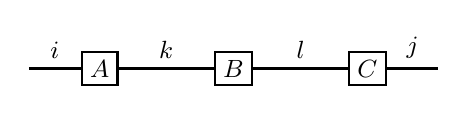
\begin{tikzpicture}[font=\small, >=Stealth]
    \node[draw, thick, inner sep=3pt] (A) at (0,0) {$A$};
    \node[draw, thick, inner sep=3pt] (B) at (1.7,0) {$B$};
    \node[draw, thick, inner sep=3pt] (C) at (3.4,0) {$C$};
    \draw[thick] (-0.9,0) -- (A) node[midway, above] {$i$};
    \draw[thick] (A) -- (B) node[midway, above] {$k$};
    \draw[thick] (B) -- (C) node[midway, above] {$l$};
    \draw[thick] (C) -- (4.3,0) node[midway, above] {$j$};
  \end{tikzpicture}
  \vspace{0.3em}

  {\small 开口指标是 $i,j$；内部指标是 $k,l$。}
\end{frame}

\begin{frame}{两种收缩顺序}
  设 $A$ 为 $n\times p$，$B$ 为 $p\times q$，$C$ 为 $q\times m$。
  \begin{itemize}
    \item 先算 $(AB)_{iq}=A_{ik}B_{kq}$，乘法次数约为 $npq$，
      再右乘 $C$，次数约为 $nqm$。
    \item 先算 $(BC)_{pm}=B_{kl}C_{lm}$，次数约为 $pqm$，
      再左乘 $A$，次数约为 $npm$。
  \end{itemize}
  两种顺序给出同一个 $M_{ij}$，中间矩阵的尺寸却不同。
  总运算量由这些中间维数决定。
  多体物理里用张量网络，就是用局部张量和收缩顺序来避免先形成巨大的中间数组。
\end{frame}

\begin{frame}{小结}
  \begin{itemize}
    \item 秩等于指标个数。张量对每个槽线性，并且每个指标乘一个 $R$。
    \item 对称部分有 $n(n+1)/2$ 个独立分量，反对称部分有 $n(n-1)/2$ 个。
    \item 应力、电导率、惯量是二阶映射；压电需要三阶。
    \item 极坐标里 $\Gamma$ 可以非零而曲率仍为零，所以 $\Gamma$ 不是张量。
    \item 张量网络把收缩画成图。收缩顺序不改变结果，但决定中间存储。
  \end{itemize}
\end{frame}

\end{document}
